
\section{Bifurcations}
\label{sec:bifurcations}

When stability of a periodic solution changes, it occurs at \textit{bifurcation
  points} in parameter space. At bifurcation points, the solution changes
qualitatively, but knowledge of the bifurcation type allows to predict the
behaviour. The type of bifurcation is related to how the Floquet multipliers
changes at said point, and the mechanism for loss of stability for the three
most common types are shown in figure \ref{fig:bifurcation}.

Bifurcations exist for multiple dimensions, but only codimension-1 bifurcations
are treated as only one parameter varies along the branch (ie. the forcing
frequency $\omega$). Bifurcations are a feature of nonlinear systems. Further
description is found in \textcite{juel2003a} or dedicated bifurcation textbooks
like \textcite{kuznetsov2013a}. Floquet multipliers $\sigma_i$ and Floquet
exponents $\lambda_i$ are related as (as restated from eq.
\eqref{eq:floquet_relations})

\begin{equation}
  \sigma_i = e^{\lambda_i T}
\end{equation}

\begin{figure}
  \centering
  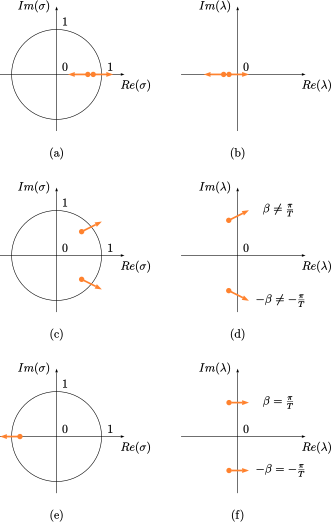
\includegraphics[width=0.7\textwidth]{bifurcation/bifurcation.pdf}
  \caption{Mechanisms for the loss of stability of a periodic solution,
    illustrated with Floquet multipliers (left column) and Floquet exponents
    (right column).
    \textbf{First row}: singular point;
    \textbf{Second row}: Neimark-Sacker bifurcation;
    \textbf{third row}: period doubling bifurcation.
    Reproduced from \parencite{detroux2016_phd}}
  \label{fig:bifurcation}
\end{figure}

\subsection{Fold and branch bifurcation Point}
\label{sec:singular_bif}

At fold point bifurcation point the state undergoes amplitude jumps and at
branch point bifurcation, branching, see below. These two types are detected when a Floquet
multiplier leaves the unit circle along the real axis through +1 or,
equivalently, when a Floquet exponent crosses the imaginary axis through 0, see
figs \ref{fig:bifurcation}(a,b)

At this point, the Jacobian matrix $\bm h_{\bm z}$ is singular: if $\bm h_{\bm
  z}$ is singular then the monodromy matrix $\bm \Phi$ of the Shooting method or
$\tilde{\bm B}$ of HB, eq \eqref{eq:hb_B}, is also singular and at least one
Floquet exponent is 0 (or a Floquet multiplier crosses the unit circle through
+1)


\begin{itemize}
\item \textit{Fold bifurcation} (also called Saddle node, Limit point or Turning
  point):\\
  The branch comes from one side and turns back, ie. the parameter($\omega$)
  increases and then decreases or decreases and then increases. Thus fold
  bifurcation indicates that there exist two solutions in its vicinity.
  It determines the upper or lower region of a bistable region and is often
  present in the vicinity of resonance peaks. This is the cause of amplitude
  jumps seen as response to stepped- or swept-sine excitation.
\item \textit{Branch bifurcation(BP)}: \\
  Two branches are connected. The two branches either meet and exchange
  stability (transcritical bifurcation), or one branch loses stability and a
  stable branch emanates from the point (pitchfork bifurcation).
\end{itemize}

Fold bifurcations satisfies
\begin{equation}
  \bm h_\omega \notin \text{range} (\bm h_{\bm z})
\end{equation}
whereas for BP
\begin{equation}
  \bm h_\omega \in \text{range} (\bm h_{\bm z})
\end{equation}

It follows that fold and BPs can be found, and distinguished, by
calculating the rank of the extended Jacobian $\bm J = [\bm h_{\bm z}| \bm
h_\omega]$ and $\bm h_{\bm z}$. If the rank of $\bm J$ is equal to $\bm h_{\bm
  z}$(and $\bm h_{\bm z}$ is singular) then it is a BP, otherwise fold.

If a BP is found, some branch switching mechanism should be used in the
continuation in order to switch branch. If no switching mechanism is used, the
continuation most likely continues on the same branch through the BP. The
new branch is found by calculating the two tangent directions at the BP;
thus some adoption of the predictor method is needed.


\subsection{Neimark-Sacker bifurcation}
\label{sec:ns_bif}

A Neimark-Sacker(NS) bifurcation (also called Hopf- or torus bifurcation) is
detected when a pair of Floquet multipliers leaves the unit circle as complex
conjugates or, equivalently, when a pair of Floquet exponent crosses the
imaginary axis as complex conjugates through any value but $\pm \frac{i\pi}{T}$,
where T is the period of oscillation, see figs \ref{fig:bifurcation}(c,d).

At NS a new type of oscillations emerges. These are called quasiperiodic
oscillations(QP) and despite the name they are not periodic. QPs contain the
forcing frequency $\omega$ (forcing), and at least another frequency
$\omega_2$(envelope). The two frequencies are incommensurate, ie.
$\frac{\omega}{\omega_2}$ is irrational. QP should not be confused with linear
beating, where the forcing frequency is close to the eigenfrequency $\omega_0$,
ie. $|\omega_0 - \omega|$ is small.

The imaginary part of the Floquet exponents that crosses the imaginary axis,
$\beta$, approximates the envelope pulsation $\omega_2$ of the QP in the
vicinity of the bifurcation, see fig. \ref{fig:bifurcation}(d)


\subsection{Period doubling bifurcation}
\label{sec:pd_bif}

A period doubling(PD) (also called flip bifurcation) is detected when a pair of Floquet
multipliers leaves the unit circle along the real axis through -1 or,
equivalently, when a pair of Floquet exponent crosses the imaginary axis as
complex conjugates through $\pm\frac{i\pi}{T}$, see figs.
\ref{fig:bifurcation}(e,f).

At PD a new branch of solution appears. The new branch have stable
periodic solutions with a doubled period. When they appear in cascade, PDs
can lead to chaos.


\section{Detecting bifurcations}
\label{sec:detecting_bifs}

To detect bifurcations during the continuation procedure, \textit{test
  functions} $\phi$ are monitored. When they change sign, a bifurcation is
detected. Each type of bifurcation have their own test function


\subsection{Fold and branch bifurcation Point}

As stated, fold and BP are characterised by rank deficiency of the
Jacobian matrix $\bm h_{\bm z}$. Thus a test function could be
\begin{equation}
  \phi_{F,BP} = \det{\bm h_{\bm z}}
\end{equation}
a computationally cheaper detection could be based on the monodromy or Hills
matrix, since this is already available
\begin{equation}
  \phi_{F,BP} = \det{\tilde{\bm B}}
\end{equation}

To distinguish between fold and BP, a dedicated test function is
\begin{equation}
  \phi_{BP} = \det
    \begin{pmatrix}
      \bm h_{\bm z} & \bm h_{\omega} \\
      \multicolumn{2}{c}{\bm t^T}
    \end{pmatrix}
\end{equation}

For detection fold bifurcation alone, a computationally cheaper way is to use
the geometric folding of the branch, ie. detect when the $\omega$ component of
the tangent prediction $\bm t$ changes sign,
\begin{equation}
  \phi_{F} = t_\omega
\end{equation}

\subsection{Neimark-Sacker and period doubling bifurcation}

NS and PD bifurcations, where a pair of Floquet exponents crosses the imaginary
axis as complex conjugates, can be detected using the \textit{bialternate
  product of a matrix} \autocite{kuznetsov2013a}. The bialternate product $\bm
P_\odot $ of a $m \times m$ matrix $\bm P$ is
\begin{equation}
  \bm P_\odot = 2\bm P \odot I_m
\end{equation}
with dimensions $m(m-1)/2$, is singular when two of its eigenvalues, $\mu 1$ and
$\mu 2$, verify:

\begin{equation}
  \mu_1 + \mu_2 = 0
\end{equation}
which is true for two purely imaginary- or real conjugate numbers. Thus the test
function is

\begin{equation}
  \phi_{NS,PD} = \det \left( \tilde{\bm B}_\odot \right)
\end{equation}
When the test function is zero, the Floquet exponents are checked. Two real
conjugates are associated with a neutral saddle point, which is not considered a
bifurcation and is ignored.
As a note: since $\tilde{\bm B}$ is diagonal, the bialternate product is also
diagonal.

\subsection{Calculating determinant efficiently}
\label{sec:bordering_tech}

Calculating the determinants needed for BP, NS and PD detection for large
scale structures might not be numerical stable. Instead the \textit{bordering
  technique} might be used, where the calculation of the determinant of $\bm G$
is replaced with calculation of a scalar function $g$ which vanishes at the same
time as the determinant \autocite{kuznetsov2013a}
\begin{equation}
  \begin{bmatrix}
    \bm G & \bm p \\
    \bm q^* & 0
  \end{bmatrix}
  \begin{bmatrix}
    \bm w \\ q
  \end{bmatrix}
  =
  \begin{bmatrix}
    \bm 0 \\ 1
  \end{bmatrix}
  \label{eq:bordered_system}
\end{equation}
where vectors $\bm p$ and $\bm q$ can be arbitrarily chosen as long as they
ensure nonsingularity of the system. This means they must be adapted or
recalculated along the branch to ensure good conditioning of the bordered
matrix.

$g$ is related to $\bm G$ by Cramer's rule
\begin{equation}
  g = \frac{\det
    \begin{pmatrix}
      \bm G & 0 \\
      \bm q^* & 1
    \end{pmatrix}}
  {\det
    \begin{pmatrix}
      \bm G & \bm p \\
      \bm q^* & 0
    \end{pmatrix}}
  =
  \frac{\det(\bm G)}
  {\det
    \begin{pmatrix}
      \bm G & \bm p \\
      \bm q^* & 0
    \end{pmatrix}}
\end{equation}


\subsection{Localisation}

When a bifurcation is detected using the test functions, the precise frequency
where it happens should be localised. To do this, a augmented system is formed
by adding the scalar test function $\phi$ to eom eq. \eqref{eq:hb_feom_compact}.

\begin{equation}
  \bm h_{aug}(\\bm z, \omega) =
  \begin{bmatrix}
    \bm h(\bm z, \omega) \\
    \phi(\bm z, \phi)
  \end{bmatrix}
  = 0
\end{equation}

The bordered technique \eqref{eq:bordered_system} is used to define the test
function $\phi$, ie. $\phi = g$ with $\bm G$ defined as: For fold and BPs, $\bm
G = \bm h_{\bm z}$. For NS and PD, $\bm G = \tilde{\bm B}_\odot$.

Thus for localising the bifurcation, the augmented system:
\begin{align}
  \label{eq:bif_aug}
  &\bm h_{aug} =
  \begin{bmatrix}
    \bm h(\bm z, \omega) \\
    g(\bm z, \phi)
  \end{bmatrix}
  = 0 \\
  &\bm J_{aug} =
  \begin{bmatrix}
    \bm h_{\bm z} & \bm h_{\omega} \\
    g_{\bm z} & g_{\omega}
  \end{bmatrix}
\end{align}
is solved using Newton-Raphson iterations. The derivatives of the test function
is needed. Using the bordered system, the derivatives are

\begin{equation}
  g_\alpha = -\bm v* \bm G_\alpha \bm w
\end{equation}
where $\alpha$ denotes one of the components of $\bm z$ or $omega$. $bm v$ and
$\bm w$ is found by solving the bordered system and its transpose, restated here:


\begin{equation}
  \begin{bmatrix}
    \bm G & \bm p \\
    \bm q* & 0
  \end{bmatrix}
  \begin{bmatrix}
    \bm w \\ q
  \end{bmatrix}
  =
  \begin{bmatrix}
    \bm 0 \\ 1
  \end{bmatrix}, \quad
    \begin{bmatrix}
    \bm G & \bm p \\
    \bm q* & 0
  \end{bmatrix}*
  \begin{bmatrix}
    \bm v \\ q
  \end{bmatrix}
  =
  \begin{bmatrix}
    \bm 0 \\ 1
  \end{bmatrix}
  \label{eq:bordered_system2}
\end{equation}
Thus only $G_\alpha$ needs to be calculated.

For fold and BPs,
\begin{equation}
  G_\alpha = \bm h_{\bm z \alpha}
\end{equation}
where $\bm h_{\bm z \alpha}$ is the derivative of the Jacobian $\bm h_z$ wrt.
$\alpha$, calculated by finite difference. When $\alpha = z_1,...,z_{(2N_H
  +1)n}$, $\bm h_{\bm z \bm z}$ is the Hessian matrix.

For NS and PD, properties of the bialternate product gives:
\begin{equation}
  \bm G_\alpha = \frac{\p}{\p \alpha} \left( \tilde{\bm B}_\odot \right) =
  \left( \frac{\p}{\p \alpha} \tilde{\bm B}_\odot \right) =
  \begin{bmatrix}
    \frac{\p \tilde{\lambda}_1}{\p \alpha} \\
    & \frac{\p \tilde{\lambda}_2}{\p \alpha} \\
    & & \ddots \\
    & & & \frac{\p \tilde{\lambda}_{2n}}{\p \alpha}
  \end{bmatrix}_\odot
\end{equation}

Instead of calculating the derivatives of the Floquet exponents by finite
difference, which would require calculating the eigenvalues of $\bm B$ for each
perturbation of the components of $\bm z$ and $\omega$, $(2N_H+1)n + 1$
evaluations, the properties of eigenvalues derivatives is
used~\autocite{aa2007a}

\begin{equation}
  \label{eq:eigen_deriv}
  \frac{\p \tilde{\lambda}_i}{\p \alpha} =
  \left( \bm \Lambda^{-1} \frac{\p \bm B}{\p \alpha} \bm \Lambda \right)_{\xi_i, \xi_i}
\end{equation}
where $\bm \Lambda$ is the matrix of right eigenvectors of $\bm B$ and $\xi_i$
is a indexation vector containing the index of the $2n$ Floquet exponents
$\tilde{\bm \lambda}$ among the eigenvalues $\bm B$(ie.
$\tilde{\lambda}_i=\lambda_{\xi_i}$).
An analytic expression for $\frac{\p \bm B}{\p \alpha}$ can then be found from
\eqref{eq:hb_B}.

Eq \eqref{eq:eigen_deriv} is valid as long as there is no repeated eigenvalues,
which is verified for most situations except when a pair of complex conjugates
turn into a pair of real eigenvalues. Since this transition occurs quickly, it
is reasonable to assume \eqref{eq:eigen_deriv} is valid. For scenarios with
repeated eigenvalues, other expressions can be found in~\autocite{aa2007a}.

Remark that $\bm h_{\bm z \alpha}$ is a zero matrix for all components in $\bm
z$ related to linear dof/Fourier coefficients. Thus it is not necessary to
evaluate all $(2N_H+1)n +1$ terms $g_\alpha$, but only the $(2N_H+1)n_{red} +1$
where $n_{red}$ is related to nonlinear dofs.


\subsection{Example}
\label{sec:bif_example}

The bifurcations for the coupled duffing system \eqref{eq:2dof} is shown in
figure \ref{fig:bif_example}. Fold, BP and NS bifurcations are found along the
branch. As expected fold bifurcations are found close to the two resonance
peaks. In fig. \ref{fig:bif_example}(b) a branch of periodic solutions emerges
from a BP bifurcation. In fig \ref{fig:bif_example}(c) QP oscillations appears
after a NS bifurcation.

\begin{figure}[ht!]
  \centering
    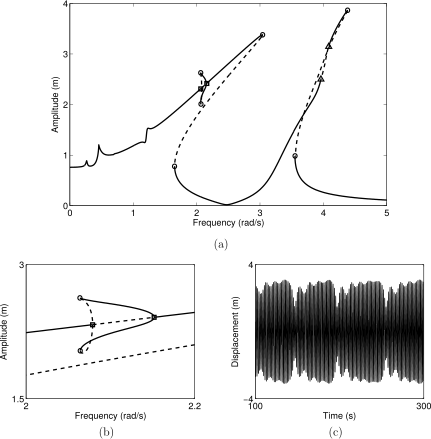
\includegraphics[width=0.85\textwidth]{bifurcation/bif_duffing.pdf}
  \caption{Bifurcation analysis of the coupled Duffing system at $x_1$ for
    $f=2$N.
    \textbf{(a)} Stable and unstable solutions are represented with solid and
    dashed lines. Fold, BP and NS bifurcations are represented with $\bm \circ$,
    $\bm \square$ and $\bm \triangle$ markers, respectively.
    \textbf{(b)} Close-up of the NRFC in the vicinity of the BPs and the
    emerging branch.
    \textbf{(c)} QP oscillations for a forcing frequency of $\omega=4$ rad/s.}
  \label{fig:bif_example}
\end{figure}

The evaluation of test functions for BP bifurcations along the branch is shown
in fig. \ref{fig:bif_BPtestfunction}. In fig \ref{fig:bif_BPtestfunction}(c) it
seen that the test function based on the determinant become very large close to
singular points whereas the bordering technique produce numerical stable values.

\begin{figure}[ht!]
  \centering
  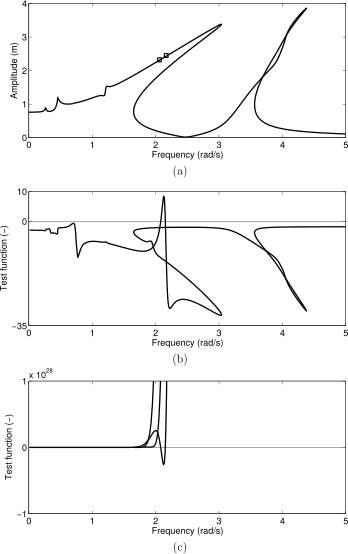
\includegraphics[width=0.85\textwidth]{bifurcation/test_funcBP.pdf}
  \caption{Test functions for BP detection.
    \textbf{(a)} NRFC and BP bifurcations marked by $\square$;
    \textbf{(b)} test function based on the bordering technique;
    \textbf{(c)} test function based on the determinant. It is noted that the
    determinant gets higher than $10^{28}$. The machine precision for a
    double precision 64 bit number is $\epsilon = 2^{-52} \sim 10^{-16}$,
    which means that the maximum spacing between two (normalised) numbers can be
    at max $2\epsilon |x|$ in order to be represented correct.}
  \label{fig:bif_BPtestfunction}
\end{figure}

\subsection{Summary}
\label{sec:bif_summary}

Bifurcation analysis can help understand nonlinear phenomena such as amplitude
jumps, quasiperiodic oscillations and period doubling. They are found during
continuation by using test functions; a summary is shown in fig
\ref{fig:bif_scheme} for Hills method.

\begin{figure}[ht!]
  \centering
 \begin{mdframed}
    \begin{enumerate}
    \item Detection of \textit{fold bifurcation}:\\
      \begin{equation*}
        \phi_F = t_{w}
      \end{equation*}
    \item Detection of \textit{bifurcation point} (BP):\\
      \begin{equation*}
        \phi_{BP} = g_{bp}
      \end{equation*}
      from the bordering system in eq. \ref{eq:bordered_system} with
      \begin{equation*}
        \bm G_{BP}
        \begin{bmatrix}
          \bm h_{\bm z} & \bm h_{\omega} \\
          \multicolumn{2}{c}{\bm t^T}
        \end{bmatrix}
      \end{equation*}
    \item Detection of \textit{Neimark-Sacker} (NS) and \textit{period doubling}
      (PD) bifurcations:\\
      \begin{equation*}
        \phi_{NS,PD} = g_{NS,PD}
      \end{equation*}
      from the bordering system in eq. \ref{eq:bordered_system} with $\bm
      G_{NS,PD} = \tilde{\bm B}_\odot$. When $\phi_{NS,PD} = 0$, matrix
      $\tilde{\bm B}$ has $\mu_1$ and $\mu_2$ among its eigenvalues, with
      \begin{equation*}
        \mu_1 + \mu_2 = 0
      \end{equation*}
      \begin{itemize}
      \item If $\mu_{1,2}=\pm i\beta$ with $\beta \neq \pi/T$, a NS
        bifurcation is detected.
      \item If $\mu_{1,2}=\pm i\beta$ with $\beta = \pi/T$, a PD bifurcation is
        detected.
      \item If $\mu_{1,2}=\pm \beta$ a neutral saddle point is detected.
      \end{itemize}
    \end{enumerate}
    \end{mdframed}
    \caption{Test functions for detection of codimensional-1 bifurcation of NFRCs}
    \label{fig:bif_scheme}
\end{figure}

%%% Local Variables:
%%% mode: latex
%%% TeX-master: "../../report"
%%% End:
